\chapter{Grafiekskes}\label{ch:grafiekskes}

\begin{figure}
	\centering
	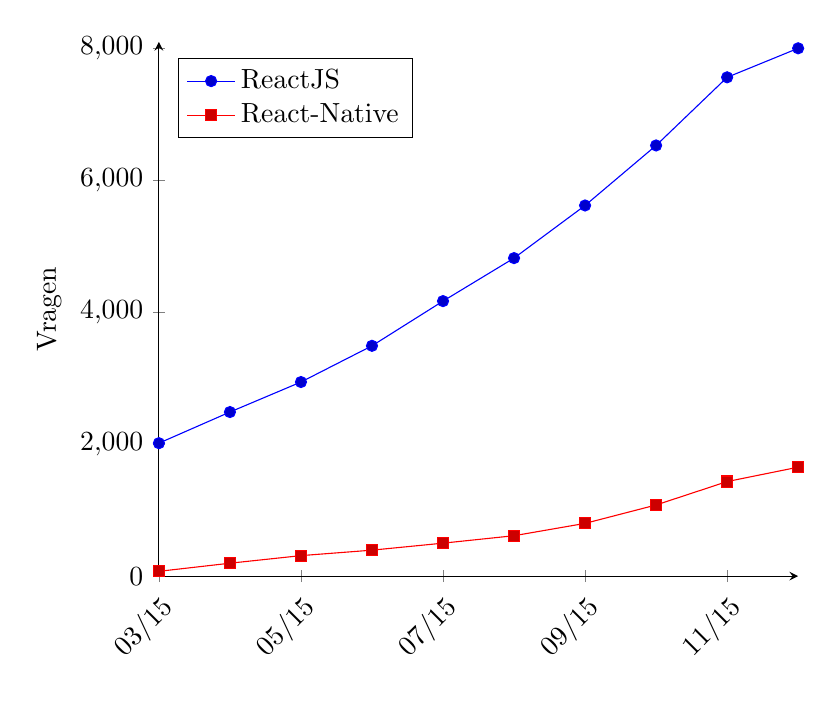
\begin{tikzpicture}
		\begin{axis}[
									symbolic x coords={03/15,04/15,05/15,06/15,07/15,08/15,09/15,10/15,11/15,12/15},
									width=.8\linewidth,
									ylabel={Vragen},
									legend cell align=left,
									ymin=0,
									ymax=8100,
									scaled ticks=false,
									axis lines=left,
									x tick label style={rotate=45, anchor=north east, inner sep=1mm},
									legend entries={ReactJS, React-Native},
									legend pos = north west
								]
			\addplot coordinates { (03/15, 2016) (04/15, 2488) (05/15, 2943) (06/15, 3492) (07/15, 4170) (08/15, 4822) (09/15, 5620) (10/15, 6530) (11/15, 7563) (12/15, 8003) };
			\addplot coordinates { (03/15, 73) (04/15, 196) (05/15, 311) (06/15, 394) (07/15, 500) (08/15, 613) (09/15, 800) (10/15, 1079) (11/15, 1434) (12/15, 1652) };
		\end{axis}
	\end{tikzpicture}
	\caption{Vragen}
	\label{fig:questions}
\end{figure}

\begin{figure}
	\centering
	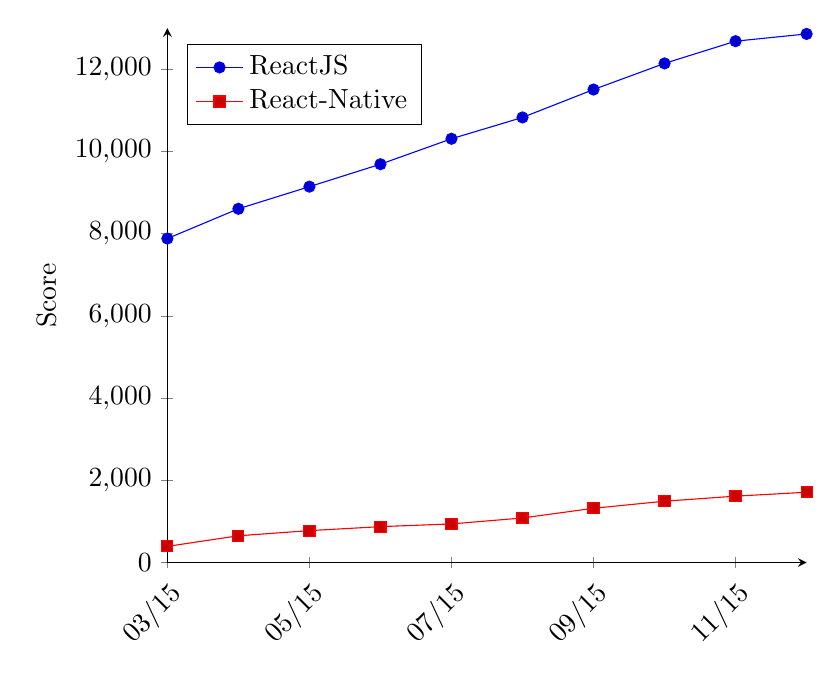
\begin{tikzpicture}
		\begin{axis}[
									symbolic x coords={03/15,04/15,05/15,06/15,07/15,08/15,09/15,10/15,11/15,12/15},
									width=.8\linewidth,
									ylabel={Score},
									legend cell align=left,
									ymin=0,
									ymax=13000,
									scaled ticks=false,
									axis lines=left,
									x tick label style={rotate=45, anchor=north east, inner sep=1mm},
									legend entries={ReactJS, React-Native},
									legend pos = north west
								]
			\addplot coordinates { (03/15, 7882) (04/15, 8606) (05/15, 9145) (06/15, 9691) (07/15, 10310) (08/15, 10829) (09/15, 11508) (10/15, 12144) (11/15, 12685) (12/15, 12861) };
			\addplot coordinates { (03/15, 392) (04/15, 650) (05/15, 775) (06/15, 872) (07/15, 938) (08/15, 1083) (09/15, 1319) (10/15, 1491) (11/15, 1614) (12/15, 1709) };
		\end{axis}
	\end{tikzpicture}
	\caption{Score}
	\label{fig:score}
\end{figure}

\begin{figure}
	\centering
	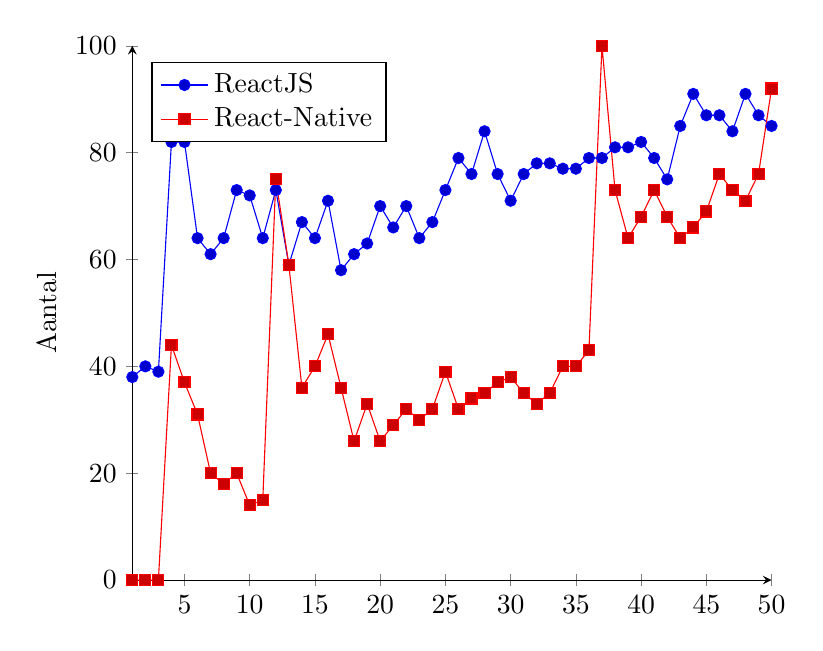
\begin{tikzpicture}
		\begin{axis}[
									xtick={0,5,...,50},
									width=.8\linewidth,
									ylabel={Aantal},
									legend cell align=left,
									ymin=0,
									ymax=100,
									scaled ticks=false,
									axis lines=left,
									legend entries={ReactJS, React-Native},
									legend pos = north west
								]
			\addplot coordinates { (1, 38) (2, 40) (3, 39) (4, 82) (5, 82) (6, 64) (7, 61) (8, 64) (9, 73) (10, 72) (11, 64) (12, 73) (13, 59) (14, 67) (15, 64) (16, 71) (17, 58) (18, 61) (19, 63) (20, 70) (21, 66) (22, 70) (23, 64) (24, 67) (25, 73) (26, 79) (27, 76) (28, 84) (29, 76) (30, 71) (31, 76) (32, 78) (33, 78) (34, 77) (35, 77) (36, 79) (37, 79) (38, 81) (39, 81) (40, 82) (41, 79) (42, 75) (43, 85) (44, 91) (45, 87) (46, 87) (47, 84) (48, 91) (49, 87) (50, 85) };
			\addplot coordinates { (1, 0) (2, 0) (3, 0) (4, 44) (5, 37) (6, 31) (7, 20) (8, 18) (9, 20) (10, 14) (11, 15) (12, 75) (13, 59) (14, 36) (15, 40) (16, 46) (17, 36) (18, 26) (19, 33) (20, 26) (21, 29) (22, 32) (23, 30) (24, 32) (25, 39) (26, 32) (27, 34) (28, 35) (29, 37) (30, 38) (31, 35) (32, 33) (33, 35) (34, 40) (35, 40) (36, 43) (37, 100) (38, 73) (39, 64) (40, 68) (41, 73) (42, 68) (43, 64) (44, 66) (45, 69) (46, 76) (47, 73) (48, 71) (49, 76) (50, 92) };
		\end{axis}
	\end{tikzpicture}
	\caption{Google Week}
	\label{fig:google}
\end{figure}